%%%%%%%%%%%%%%%%%%%%%%%%%%%%%%%%%%%%%%%%%%%%%%%%%%%%%%%%%%%%
%%  This Beamer template was created by Cameron Bracken.
%%  Anyone can freely use or modify it for any purpose
%%  without attribution.
%%
%%  Last Modified: January 9, 2009
%%

\documentclass[xcolor=x11names,compress]{beamer}

%% General document %%%%%%%%%%%%%%%%%%%%%%%%%%%%%%%%%%
\usepackage{graphicx}
\usepackage{tikz}
\usetikzlibrary{decorations.fractals}
%%%%%%%%%%%%%%%%%%%%%%%%%%%%%%%%%%%%%%%%%%%%%%%%%%%%%%

%% add by Tianyi @ UNH
\definecolor{unhblue}{rgb}{0.149,.251,.545}

%% Beamer Layout %%%%%%%%%%%%%%%%%%%%%%%%%%%%%%%%%%
\useoutertheme[subsection=false,shadow]{miniframes}
\useinnertheme{default}
\usefonttheme{serif}
\usepackage{palatino}

\setbeamerfont{title like}{shape=\scshape}
\setbeamerfont{frametitle}{shape=\scshape}

\setbeamercolor*{lower separation line head}{bg=unhblue} 
\setbeamercolor*{normal text}{fg=black,bg=white} 
\setbeamercolor*{alerted text}{fg=red} 
\setbeamercolor*{example text}{fg=black} 
\setbeamercolor*{structure}{fg=black} 
 
\setbeamercolor*{palette tertiary}{fg=black,bg=black!10} 
\setbeamercolor*{palette quaternary}{fg=black,bg=black!10} 

\renewcommand{\(}{\begin{columns}}
\renewcommand{\)}{\end{columns}}
\newcommand{\<}[1]{\begin{column}{#1}}
\renewcommand{\>}{\end{column}}
%%%%%%%%%%%%%%%%%%%%%%%%%%%%%%%%%%%%%%%%%%%%%%%%%%




\begin{document}


%%%%%%%%%%%%%%%%%%%%%%%%%%%%%%%%%%%%%%%%%%%%%%%%%%%%%%
%%%%%%%%%%%%%%%%%%%%%%%%%%%%%%%%%%%%%%%%%%%%%%%%%%%%%%
\section{\scshape Motivation}
\begin{frame}
\title{ Online Policy Training vs Heuristic Search Using
  Reinforcement Learning to Avoid Dynamic Obstacles}
%Efficient Online Path Planning by Heuristic Training using Reinforcement Learning
\subtitle{cs980 project}
\author{
	Tianyi Gu, Mostafa Hussein, Yishan Luo, Yuncong Zhou\\
	%{\it Humboldt State University}\\
        
\includegraphics[height=0.4in]{figures/unh-logo-words.eps} 
        \vspace{-0.1in}\\
        %Department of Computer Science\\~
}
\date{
	% \begin{tikzpicture}[decoration=Koch curve type 2] 
	% 	\draw[DeepSkyBlue4] decorate{ decorate{ decorate{ (0,0) -- (3,0) }}}; 
	% \end{tikzpicture}  
	% \\
	% \vspace{1cm}
	\today
}
\titlepage
\end{frame}

%%%%%%%%%%%%%%%%%%%%%%%%%%%%%%%%%%%%%%%%%%%%%%%%%%%%%%
%%%%%%%%%%%%%%%%%%%%%%%%%%%%%%%%%%%%%%%%%%%%%%%%%%%%%%
\begin{frame}{Motivation}
\begin{itemize}
\item Avoid dynamic obstacles is crucial 
\begin{itemize}
\item Autonomous vehicle navigation
\item Indoor robot navigation
\end{itemize}
\end{itemize}
\end{frame}

%%%%%%%%%%%%%%%%%%%%%%%%%%%%%%%%%%%%%%%%%%%%%%%%%%%%%%
%%%%%%%%%%%%%%%%%%%%%%%%%%%%%%%%%%%%%%%%%%%%%%%%%%%%%%
\section{\scshape Problem}
\subsection{Online Policy Training}
\begin{frame}{Online Policy Training}
\begin{itemize}
\item Given start state, goal state, and static obstacles
\item Compute online policy based on observation of dynamic obstacles
\end{itemize}
\begin{figure}
\centering
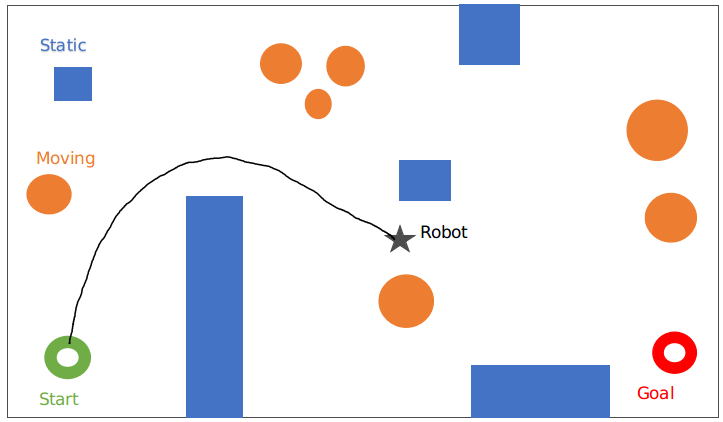
\includegraphics[width=0.8\textwidth]{./figures/problem1.png}
\end{figure}
\end{frame}

%%%%%%%%%%%%%%%%%%%%%%%%%%%%%%%%%%%%%%%%%%%%%%%%%%%%%%
%%%%%%%%%%%%%%%%%%%%%%%%%%%%%%%%%%%%%%%%%%%%%%%%%%%%%%

\begin{frame}{Online Policy Training: MDP}
\begin{itemize}
\item MDP:
\begin{itemize}
\item States: grid world states
\item Actions: up, down, left, right
\item Rewards: goal: 1, collision: -1000
\item Transition: Unknown
\end{itemize}
\only<1>{
\begin{figure}
\centering
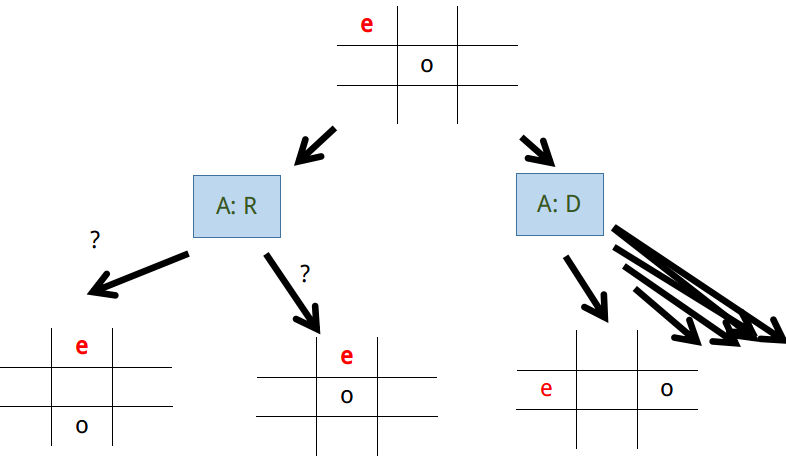
\includegraphics[width=0.8\textwidth]{./figures/tree.png}
\end{figure}
}
\pause
\item Approach:
\begin{itemize}
\item TD($\lambda$), Q learning, Sarsa
\item Monte Carlo Tree Search
\end{itemize}
\end{itemize}
\vspace{-0.1in}
\begin{figure}
\centering
\begin{tabular}{c c}
    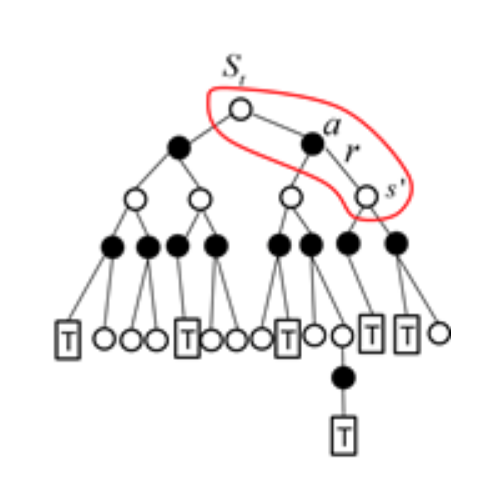
\includegraphics[width=0.4\textwidth]{./figures/td0.png}&
    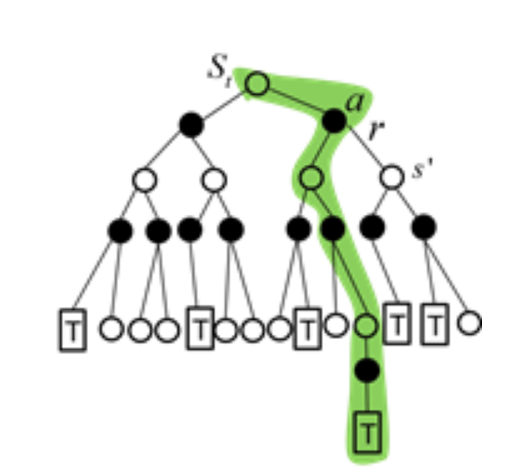
\includegraphics[width=0.4\textwidth]{./figures/mc.png}
\end{tabular}
\end{figure}
\end{frame}

%%%%%%%%%%%%%%%%%%%%%%%%%%%%%%%%%%%%%%%%%%%%%%%%%%%%%%
%%%%%%%%%%%%%%%%%%%%%%%%%%%%%%%%%%%%%%%%%%%%%%%%%%%%%%

\begin{frame}{Online Path Planning}
\begin{itemize}
\item Real Time Heuristic Search
\begin{itemize}
\item estimate obstacles' movement
\item deterministic problem with different cost function
\end{itemize}
\pause
\item Approach:
\begin{itemize}
\item Greedy, A*
\item LSS-LRTA*
\end{itemize}
\end{itemize}
\begin{figure}
\centering
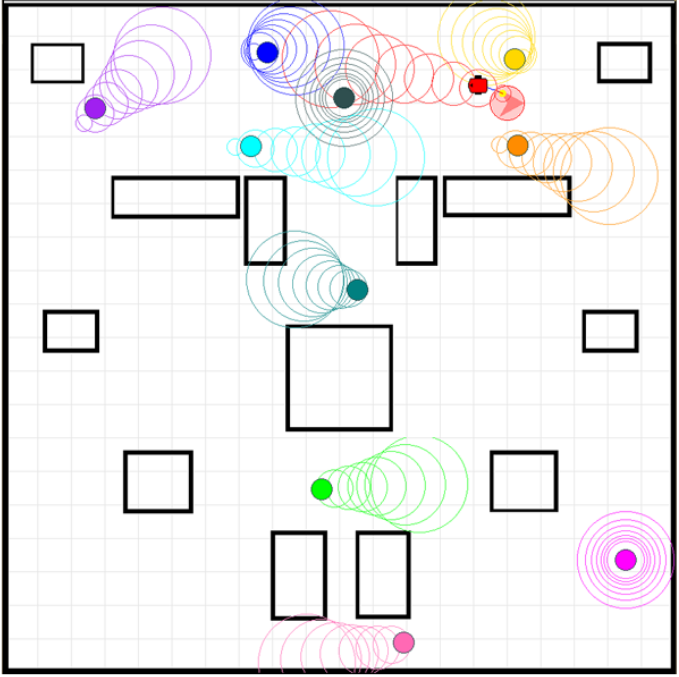
\includegraphics[width=0.5\textwidth]{./figures/rts.png}
\end{figure}
\end{frame}

%%%%%%%%%%%%%%%%%%%%%%%%%%%%%%%%%%%%%%%%%%%%%%%%%%%%%%
%%%%%%%%%%%%%%%%%%%%%%%%%%%%%%%%%%%%%%%%%%%%%%%%%%%%%%
\section{\scshape Experiment}
\begin{frame}{Experiment}
\begin{itemize}
\item Compare Policy Training vs Heuristic Search
\item Theoretically prove the value functions are the same
\end{itemize}
\begin{figure}
\centering
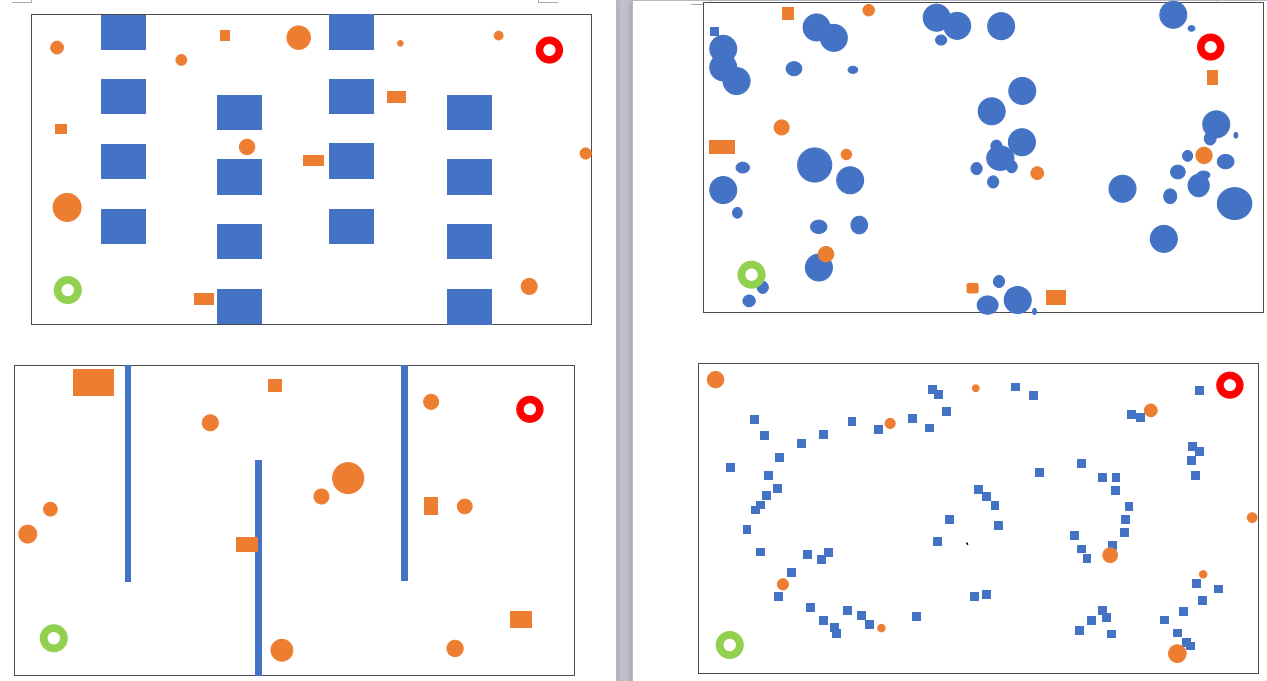
\includegraphics[width=\textwidth]{./figures/exps.png}
\end{figure}
\end{frame}

%%%%%%%%%%%%%%%%%%%%%%%%%%%%%%%%%%%%%%%%%%%%%%%%%%%%%%
%%%%%%%%%%%%%%%%%%%%%%%%%%%%%%%%%%%%%%%%%%%%%%%%%%%%%%

\end{document}